\documentclass[a4paper]{scrreprt}

% Uncomment to optimize for double-sided printing.
% \KOMAoptions{twoside}

% Set binding correction manually, if known.
% \KOMAoptions{BCOR=2cm}

% Localization options
\usepackage[english]{babel}
\usepackage[T1]{fontenc}
\usepackage[utf8]{inputenc}

% PDF-compatible landscape mode.
% Makes PDF viewers show the page rotated by 90°.
\usepackage{pdflscape}

% Advanced tables
\usepackage{tabularx}

% Fancy tablerules
\usepackage{booktabs}

% Current time
\usepackage[useregional=numeric]{datetime2}

% Float barriers.
% Automatically add a FloatBarrier to each \section
\usepackage[section]{placeins}

% \usepackage{geometry}
% \usepackage{layout}

% Math tools
\usepackage{mathtools}
% Math symbols
\usepackage{amsmath,amsfonts,amssymb}
\usepackage{amsthm}
% General symbols
\usepackage{stmaryrd}

% Utilities for quotations
\usepackage{csquotes}

% Bibliography
\usepackage[
  style=alphabetic,
  backend=biber, % Default backend, just listed for completness
  sorting=ynt % Sort by year, name, title
]{biblatex}
\addbibresource{references.bib}

% Source code & highlighting
\usepackage{listings}

% SI units
\usepackage{siunitx}

\newcommand{\lecture}{41506 - Seminar Cryptography and Data Security}
% Convenience commands
\newcommand{\mailsubject}{\lecture - Report}
\newcommand{\maillink}[1]{\href{mailto:#1?subject=\mailsubject}
                               {#1}}

% Should use this command wherever the print date is mentioned.
\newcommand{\printdate}{\today}

\subject{\lecture}
\title{Punchscan: Digital voting scheme with paper-based receipts}

\author{Michael Senn \maillink{michael.senn@students.unibe.ch} --- 16-126-880}

\date{\printdate}

% Needs to be the last command in the preamble, for one reason or
% another. 
\usepackage{hyperref}

% Custom aliases used throughout
\newcommand{\ptop}{$\pi_{\text{top}}$}
\newcommand{\pbottom}{$\pi_{\text{bottom}}$}
\newcommand{\ctop}{$Com(\pi_{\text{top}})$}
\newcommand{\cbottom}{$Com(\pi_{\text{bottom}})$}

\begin{document}

\maketitle

\begin{abstract}
	Lorem ipsum dolor si amet, et coniunctur.
\end{abstract}

\chapter{Introduction}
\label{chapter:introduction}

In the course of history, many different voting systems have been designed and
used. They differ in their trust models, their usability and other aspects. In
the last decades, ongoing digitalization has also influenced election systems
in that electronic systems have started to play a role in the voting process.

One such system is Punchscan, published in the early 2000s. It is a voting
system using paper ballots, yet heavily relies on cryptographic operations to
provide voter privacy, resilience towards malicious parties, and individual
verifiability. This report aims to provide an overview of Punchscan's
workings and shortcomings.

Chapter \ref{ch:ballot_design_and_voting} will start by discussing the ballot
layout as well as the voting process from the point of view of the voter.
Chapter \ref{ch:setup} will describe the work performed by the election
authority and auditors ahead of time. Chapter \ref{ch:tally} will describe the
tally phase including its audits. Finally chapter \ref{ch:security} will
discuss the integrity and privacy goals --- as well as how and if they are
achieved --- of Punchscan. 

% TODO don't like this sentence
The report is heavily based on the introductory paper to Punchscan by Fisher et
al.\autocite{fisherPunchscanIntroductionSystem2006}, with other work being
referenced where appropriate.

\section{Involved parties}

People participating in the Punchscan election system can be grouped into one
of three categories.
\begin{description}
\item[Voters] Voters participate in the election. They are assumed to be able
to authenticate themselves towards the election authority. Malicious voters may
attempt to learn of others' votes, or sell their own vote to third parties.
\item[Election authority] The election authority consists of a single person
--- or a set of persons in a threshold setting --- which handles the setup and
tally phases of the election. A malicious election authority may attempt to
influence the outcome of the election. In a broader sense the election
authority also includes poll workers assisting voters. The election authority
is assumed to be able to generate key material at will, and share it
securely with other parties where required.
\item[Auditors] Auditors are a set of people tasked with ensuring vote
integrity. At least one auditor is assumed to be honest.
\end{description}

\section{Notation and terminology}

\subsection{Permutations}

Permutations will be denoted by the letter $\pi$, with an index describing
their purpose. As an example, $\pi_{top}$ will be used to refer to the
permutation of the ballot's top page. The standard one-line notation will be
used, where $\pi = cba$ refers to a permutation $\pi$ such that $\pi(a) = c,
\pi(b) = b, \pi(c) = a$. For permutations over two elements the notation from
the Punchscan paper is adopted, where $\rightarrow$ is the identity permutation
and $\circlearrowright$ is the permutation flipping the two elements.
Composition of permutations is denoted as $\pi_1 \circ \pi_2$, evaluated
right-to-left.

\subsection{Representation of data}

The Punchscan system generates and manipulates a fair bit of data, which will
be described in terms of relational databases such as `tables', `rows',
`columns', `primary keys', `foreign keys' and so on. This does not imply a
requirement for specific implementations of Punchscan to use a relational
storage system, although no clear benefit to using non-relational storage is
apparent as the data is inherently relational.

\chapter{Ballot design and voting}
\label{ch:ballot_design_and_voting}

\section{Ballot design}

A Punchscan ballot consists of two pages stacked atop each other, as shown in
figure \ref{fig:punchscan_ballot}. It is uniquely identified by a numerical ID
printed on both pages. The top page contains the questions asked as well as all
possible answers. Each answer is mapped to a symbol --- in this case the
letters `a', `b' and `c'. The bottom page contains the same symbols, which can
be seen through cutouts in the top page when stacked atop each other. Both the
mapping of answers to symbols on the top page, as well as the order of symbols
on the bottom page, are independent random permutations per ballot. Multiple
questions can also be printed on the same ballot without loss of functionality
or privacy, as will be discussed later.

\begin{figure}[h]
\centering
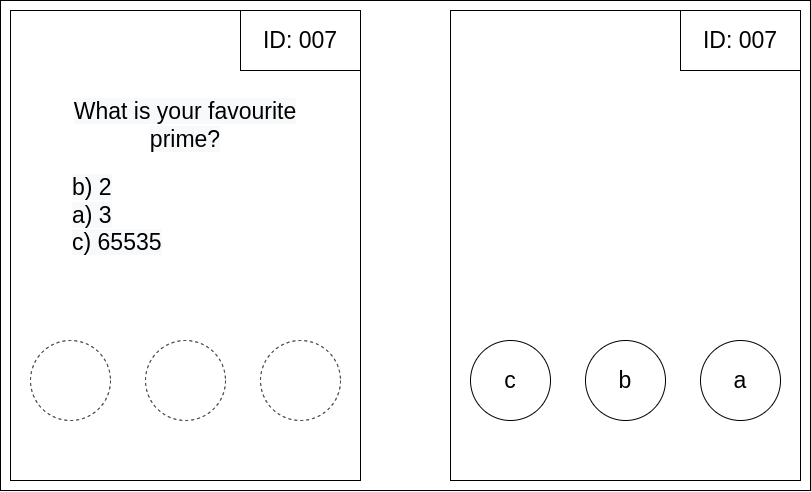
\includegraphics[width=0.7\textwidth]{../resources/high_level_ballot.drawio}
\caption{Punchscan ballot consisting of top (left) and bottom (right) page}
\label{fig:punchscan_ballot}
\end{figure}

\section{Voting process}

After having identified themselves at the polling place, a voter will have to
commit to getting to keep either the top or the bottom page of the ballot as a
receipt. They will then receive a random ballot, consisting of a top and bottom
page stuck together and enter the voting booth.

Within, the voter will read the question and decide on their answer. They will
look up which symbol their choice maps to on the top page, and then look
through which hole on the top page the corresponding symbol printed on the
bottom page is visible. They will then mark the corresponding slot using a
dauber --- a huge highlighter as used in Bingo --- thereby leaving a stain on
both the top as well as the bottom page of the ballot. The effect of having
marked their choice is shown in figure \ref{fig:punchscan_ballot_voted}.

The voter will then destroy the half of the ballot they will not keep by
feeding it through a shredder. They then exit the voting booth, and hand the
remaining half to a poll worker. The poll worker will scan the page, and feed
it through an OCR software. The voter gets to see and confirm that the scanned
page, including the detected choice, matches their physical copy. If so they
get to leave, keeping their scanned half of the ballot as a receipt.

\begin{figure}
\centering
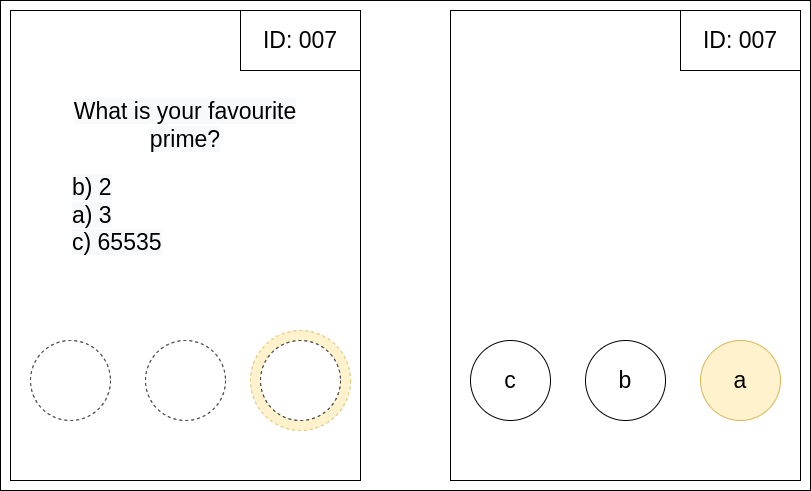
\includegraphics[width=0.7\textwidth]{../resources/high_level_ballot_voted_split.drawio}
\caption{Top (left) and bottom (right) pages of ballot after voter chose `3' as their favourite prime}
\label{fig:punchscan_ballot_voted}
\end{figure}

\chapter{Setup}
\label{ch:setup}

During the setup phase the election authority will initialize the contents of
three tables. This will be followed by an audit to ensure honesty of the
election authority. The three tables which are initialized are referred to as
the \textbf{P}, \textbf{D} and \textbf{R} tables:
\begin{description}
\item[\emph{P}rint table] The print table contains all information which is
	required to print the ballots, along with information for auditing
		purposes.
\item[\emph{D}ecryption table] The decryption table contains all information
	required to decrypt the voter's encrypted vote in the tally phase,
		along with information for auditing purposes.
\item[\emph{R}esults table] The results table contains the outcome of election.
\end{description}

For the following we will assume an election with one question and two answers
$a$ and $b$, voted on by $n$ voters.

\section{Election authority in a threshold setting}

For the purpose of this chapter we assume the election authority to be a single
entity, in full possession of their private keys. In a real-life deployment it
would be prudent to utilize some form of threshold cryptography to spread this
trust across multiple parties.

\section{Initializing the \textbf{P} table}

The election authority first populates $2n$ rows of the \textbf{P} table as shown
in table \ref{tbl:p_table_full}. This table is indexed by a primary key $ID_P$,
corresponding to the ballot ID which will be printed on both pages of the
ballot. It then picks two random permutations \ptop{} and \pbottom{},
corresponding to the permutations of the top and bottom pages respectively.
Permutations will be shown explicitly. In an actual implementation they might
however be chosen as shown in section \ref{sec:generating_permutations}. The
\emph{Choice} column is left empty, and will be used to store the voter's
permuted choice later on.

For each row it then calculates two cryptographic commitments, \ctop{} and
\cbottom{}, to \ptop{} and \pbottom{} respectively. The utilized commitment
scheme is described in section \ref{sec:commitment_scheme}.

\begin{table}
	\centering
	\begin{tabular}{|c|c|c|c|c|c|}
		\hline
		$ID_P$ & \ptop & \pbottom & $Choice$ & \ctop & \cbottom \\
		\hline
		1 & ab & ab & & $C_{1, 1}$ & $C_{1, 2}$ \\
		2 & ab & ba & & $C_{2, 1}$ & $C_{2, 2}$ \\
		3 & ba & ab & & $C_{3, 1}$ & $C_{3, 2}$ \\
		4 & ba & ba & & $C_{4, 1}$ & $C_{4, 2}$ \\
		5 & ab & ba & & $C_{5, 1}$ & $C_{5, 2}$ \\
		6 & ba & ab & & $C_{6, 1}$ & $C_{6, 2}$ \\
		\hline
	\end{tabular}
	\caption{Print table}
	\label{tbl:p_table_full}
\end{table}

\section{Initializing the \textbf{D} table}

The election authority then populates $2n$ rows of the \textbf{D} table as per
table \ref{tbl:d_table_full}. This table contains a reference to the \textbf{P}
table by means of the $ID_P$ column, and to the \textbf{R} table by means of
the $ID_R$ column. Both $ID_P$ and $ID_R$ are random and independent
permutations of the elements $1, 2, \ldots, 2n$. It then chooses \pone{}
randomly, and calculates \ptwo{} such that $\ptwo \circ \pone \circ \pbottom
\circ \ptop = id$ yields the identity permutation.  The $\hat{R}$ column is
left empty during the setup phase and will be used during decryption. 

Finally a  cryptographic commitment $Com_i$ to each row is generated, as well
as two cryptographic commitments $Com_{ID_P, \pone}$ to the content of columns
$ID_P$ and \pone{}, and $Com_{\ptwo, ID_R}$ to the content of columns \ptwo{}
and $ID_R$.

\begin{table}[h]
	\begin{subtable}{.6\linewidth}
		\centering
		\begin{tabular}{|c|c|c|c|c|c|}
			\hline
			$ID_P$ & $\pi_1$ & $\hat{R}$ & $\pi_2$ & $ID_R$ & $Com_{i}$ \\
			\hline
			6 & $\rightarrow$       & & $\circlearrowright$ & 5 & $C_6$ \\
			5 & $\circlearrowright$ & & $\rightarrow$       & 4 & $C_5$ \\
			2 & $\circlearrowright$ & & $\rightarrow$       & 1 & $C_2$ \\
			1 & $\circlearrowright$ & & $\circlearrowright$ & 3 & $C_1$ \\
			4 & $\rightarrow$       & & $\rightarrow$       & 2 & $C_4$ \\
			3 & $\rightarrow$       & & $\circlearrowright$ & 6 & $C_3$ \\
			\hline
			\multicolumn{2}{|c|}{$Com_{ID_P, \pi_1}$} &   & \multicolumn{2}{c|}{$Com_{\pi_2, ID_R}$} & \\
			\hline
		\end{tabular}
		\caption{Decryption table}
		\label{tbl:d_table_full}
	\end{subtable}%
	\begin{subtable}{.4\linewidth}
		\centering
		\begin{tabular}{|c|c|}
			\hline
			$ID_R$ & $R$ \\
			\hline
			1 & \\
			2 & \\
			3 & \\
			4 & \\
			5 & \\
			6 & \\
			\hline
			\multicolumn{2}{l}{} % Ugly hack to vertically align the two tables.
		\end{tabular}
		\caption{Results table}
		\label{tbl:r_table_full}
	\end{subtable}
	\caption{Decryption and results tables}
\end{table}

\section{Initializing the \textbf{R} table}

In a last step the election authority initializes $2n$ empty rows of the
\textbf{R} table as shown in table \ref{tbl:r_table_full}.

\begin{table}
\end{table}

\section{Setup audit}

The final phase of the setup consists of a first audit by a set of trusted
auditors. The election authority reveals the primary ballot ID $ID_P$ and
commitments of the \textbf{P} table, as well as the row and column commitments
of the \textbf{D} table. The revealed data is shown in table
\ref{tbl:setup_audit}. The auditor then gets to pick $n$ rows at random, for
which the election authority will reveal the full contents, including what is
required to open the commitments. An example of a revealed table is shown in
table \ref{tbl:setup_audit_revealed}. The auditor will then verify that all row
commitments are correct, and that $\ptwo \circ \pone \circ \pbottom \circ \ptop
= id$ holds.

All rows which were fully revealed during this audit are considered spoiled,
and will not be used anymore in subsequent parts of the voting scheme.

\begin{table}[h]
	\centering
	\begin{subtable}{.5\linewidth}
		\begin{tabular}{|c|c|c|c|c|c|}
			\hline
			$ID_P$ & $\pi_{t}$ & $\pi_{b}$ & $c$ & $Com_{\pi_{t}}$ & $Com_{\pi_{b}}$ \\
			\hline
			1 & & & & $C_{1, 1}$ & $C_{1, 2}$ \\
			2 & & & & $C_{2, 1}$ & $C_{2, 2}$ \\
			3 & & & & $C_{3, 1}$ & $C_{3, 2}$ \\
			4 & & & & $C_{4, 1}$ & $C_{4, 2}$ \\
			5 & & & & $C_{5, 1}$ & $C_{5, 2}$ \\
			6 & & & & $C_{6, 1}$ & $C_{6, 2}$ \\
			\hline
		\end{tabular}
	\end{subtable}%
	\begin{subtable}{.5\linewidth}
		\begin{tabular}{|c|c|c|c|c|c|}
			\hline
			$ID_P$ & $\pi_1$ & $\hat{R}$ & $\pi_2$ & $ID_R$ & $Com_{i}$ \\
			\hline
			& & & & & $C_6$ \\
			& & & & & $C_5$ \\
			& & & & & $C_2$ \\
			& & & & & $C_1$ \\
			& & & & & $C_4$ \\
			& & & & & $C_3$ \\
			\hline
			\multicolumn{2}{|c|}{$Com_{ID_P, \pi_1}$} &   & \multicolumn{2}{c|}{$Com_{\pi_2, ID_R}$} & \\
			\hline
		\end{tabular}
	\end{subtable}
	\caption{Subset of tables released for auditing purposes}
	\label{tbl:setup_audit}
\end{table}

\begin{table}
	\centering
	\begin{subtable}{.5\linewidth}
		\begin{tabular}{|c|c|c|c|c|c|}
			\hline
			$ID_P$ & $\pi_{t}$ & $\pi_{b}$ & $c$ & $Com_{\pi_{t}}$ & $Com_{\pi_{b}}$ \\
			\hline
			1 & & & & $C_{1, 1}$ & $C_{1, 2}$ \\
			2 & ab & ba & & $C_{2, 1}$ & $C_{2, 2}$ \\
			3 & & & & $C_{3, 1}$ & $C_{3, 2}$ \\
			4 & ba & ba & & $C_{4, 1}$ & $C_{4, 2}$ \\
			5 & ab & ba & & $C_{5, 1}$ & $C_{5, 2}$ \\
			6 & & & & $C_{6, 1}$ & $C_{6, 2}$ \\
			\hline
		\end{tabular}
	\end{subtable}%
	\begin{subtable}{.5\linewidth}
		\begin{tabular}{|c|c|c|c|c|c|}
			\hline
			$ID_P$ & $\pi_1$ & $\hat{R}$ & $\pi_2$ & $ID_R$ & $Com_{i}$ \\
			\hline
			&                     & &                     &   & $C_6$ \\
			5 & $\circlearrowright$ & & $\rightarrow$       & 4 & $C_5$ \\
			2 & $\circlearrowright$ & & $\rightarrow$       & 1 & $C_2$ \\
			&                     & &                     &   & $C_1$ \\
			4 & $\rightarrow$       & & $\rightarrow$       & 2 & $C_4$ \\
			&                     & &                     &   & $C_3$ \\
			\hline
			\multicolumn{2}{|c|}{$Com_{ID_P, \pi_1}$} &   & \multicolumn{2}{c|}{$Com_{\pi_2, ID_R}$} & \\
			\hline
		\end{tabular}
	\end{subtable}
	\caption{Subset of tables released for auditing purposes}
	\label{tbl:setup_audit_revealed}
\end{table}

\section{Generating permutations}
\label{sec:generating_permutations}

Implementations of Punchscan must be able to generate permutations in such a
way that three properties hold:
\begin{itemize}
	\item Observing parts of a permutation must give an attacker no useful information about the rest of the permutation.
	\item A compact representation must exist, such that it can be stored in a database.
	\item Permutations must be generated computationally, in a way that all
		members of the election authority trust the process.
\end{itemize}

The introductory paper outlines two ways by which such permutations can be
constructed \autocite[section 8]{fisherPunchscanIntroductionSystem2006}. The
first, shown in section \ref{sec:permutations_via_symmetric_cipher} is used to
permute the rows of the $D$ and $R$ tables. The second, shown in section
\ref{sec:permutations_via_shifts} is used to permute the top and bottom pages
of the ballot.

\subsection{Generate permutation over $n$ elements using a symmetric cipher}
\label{sec:permutations_via_symmetric_cipher}

Agree on a symmetric cipher and key $K$. Start with a table with two columns.
Initialize the first column to values $1, 2, \ldots, n$. Fill the second column
with $Enc_K(1), Enc_K(2), \ldots, Enc_K(n)$, where $Enc_K(i)$ is the result of
encrypting $i$ with key $K$ --- using a standard padding scheme if required.
Sort the table by the second column using some canonical ordering. Then, the
order of the numbers in the first column defines a permutation
indistinguishable from a truly random permutation, given standard assumptions
placed on symmetric ciphers.

\subsection{Generate permutation over $n$ elements as combination of two cyclic shifts}
\label{sec:permutations_via_shifts}

For the $\pi_1, \pi_2, \pi_{top}, \pi_{bottom}$ permutations the authors note
that a simpler consruction is sufficient to generate all possible mappings
between answer possibilities and symbols. They propose to generate two random
numbers, and cyclically shift the list of answer possibilities by one of the
random numbers, and the list of answer symbols by the other. This will not
generate all possible permutations as e.g. the relative order of elements is
preserved.

\section{Commitment scheme}

The introductory paper defines their own custom commitment scheme based on the
AES block cipher\autocite[section 9]{fisherPunchscanIntroductionSystem2006}.
Let $K_1, K_2$ be two AES-128 keys. Let $C$ be a public 128-bit constant. Let
$Enc_K(m)$ denote the result of encrypting a 128-bit message $m$ using the key
$K$, $Dec_K(c)$ the result of decrypting a 128-bit ciphertext $c$ using the key
$K$. Let $||$ denote binary concatenation.

\subsection{Key-derivation function}

They first define a custom key-derivation function, shown in algorithm
\ref{alg:kdf}.

\begin{algorithm}
	\begin{algorithmic}
		\State \textbf{Input} $m$
		\State $m_{128} \gets \text{First 128 bits of } m$ \Comment{Pad with zeroes if $m$ shorter than 128 bits}
		\State $K_m \gets Dec_{K_1}(C \oplus Enc_{K_2}(C \oplus Enc_{K_1}(m_{128})))$
		\State \textbf{Return} $K_m$
	\end{algorithmic}
	\caption{$KDF(m)$}
	\label{alg:kdf}
\end{algorithm}

\subsection{Commitment scheme}

They then define a commitment scheme as shown in algorithm \ref{alg:commit}.

\begin{algorithm}
	\begin{algorithmic}
		\State \textbf{Input} $m$
		\State $K_m \gets \Call{KDF}{m}$
		\State $s \gets Enc_{K_m}(C)$
		\State $h_1 \gets \Call{SHA-256}{m || s}$
		\State $h_2 \gets \Call{SHA-256}{m || Enc_{K_m}(h_1)}$ \Comment{AES in ECB mode with PKCS\#5 padding}
		\State \textbf{Return} $(h_1, h_2)$
	\end{algorithmic}
	\caption{$Commit(m)$}
	\label{alg:commit}
\end{algorithm}

\subsection{Opening commitments}

While not described in the paper, one can surmise that opening the commitments
is done by releasing $K_m$. As generation of commitments is deterministic, this
will allow recalculating the commitment and comparing for equality.


\printbibliography

\end{document}
